\section{Exploring the resolution speed}

\subsection*{Question 3.1}
\textit{What is the average resolution speed to an incident? Resolution speed is defined as the difference between the Event Clearance Date value (moment when the police closed the file of an incident) and the At Scene Time value (moment when the police arrived at the scene of the incident).}

The dataset does not define the average resolution time explicitly.
Thus, we need to add a new columns to the dataset with this information.
Tableau is able to compute new dimensions using the existing ones.
Since we compute a difference between $2$ timestamp, we use the function ``datediff'' to get a proper result.

The average resolution time of the entire dataset is about $2$ hours.

\begin{figure}[h]
	\centering
	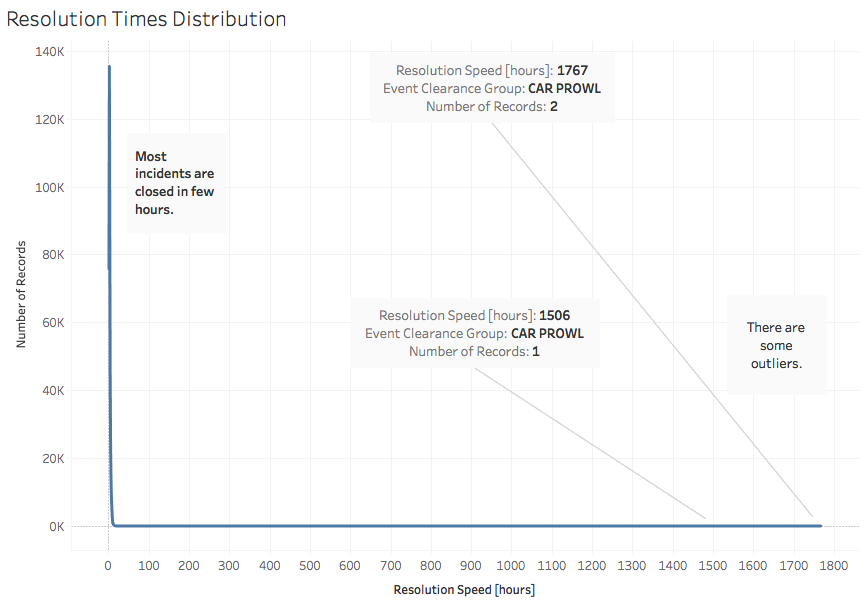
\includegraphics[width=0.9\columnwidth]{figures/3_1_resolution_speed_outliers}
	\caption{Distribution of the resolution times. The annotations on the plot show some outliers with very high resolution times. Most of the incidents are closed in few hours.}
	\label{fig:3_1_resolution_speed_outliers}
\end{figure}

\cref{fig:3_1_resolution_speed_outliers} shows the distribution of resolution times.
We can notice that:
\begin{itemize}
    \item Most incidents are closed in few hours.
    \item There are few outliers that have a resolution time of over $1500$ hours (approximately 2 months). All outliers share the same type: ``Car Prowl''.
\end{itemize}

The line chart gives already some interesting insides about incidents resolution times.
However, due to the described outliers, it is difficult to read the left part of the chart, where most of the distribution mass is.

To solve the problem, we add an histogram of the resolution times.
Resolution time is a continuos measure.
However, we are not interested in the precise value of resolution time for each incident, rather in the overall distribution.
To visualize the distribution, we discretize the resolution time in buckets of $1$ hour.
Since most of the density mass in the first $15$ buckets, we cut the histogram after the first $20$ ones.
Since we are loosing the outliers, we add a table that contains such information.

\cref{fig:3_1_resolution_speed} shows the final dashboard.
We can notice that:
\begin{itemize}
    \item The average resolution time is about $2$ hours.
    \item There are some outliers, but their number is really low in comparison to the amount of entries.
    \item Overall most incidents are closed in less than $10$ hours.
\end{itemize}

\begin{figure}[h]
	\centering
	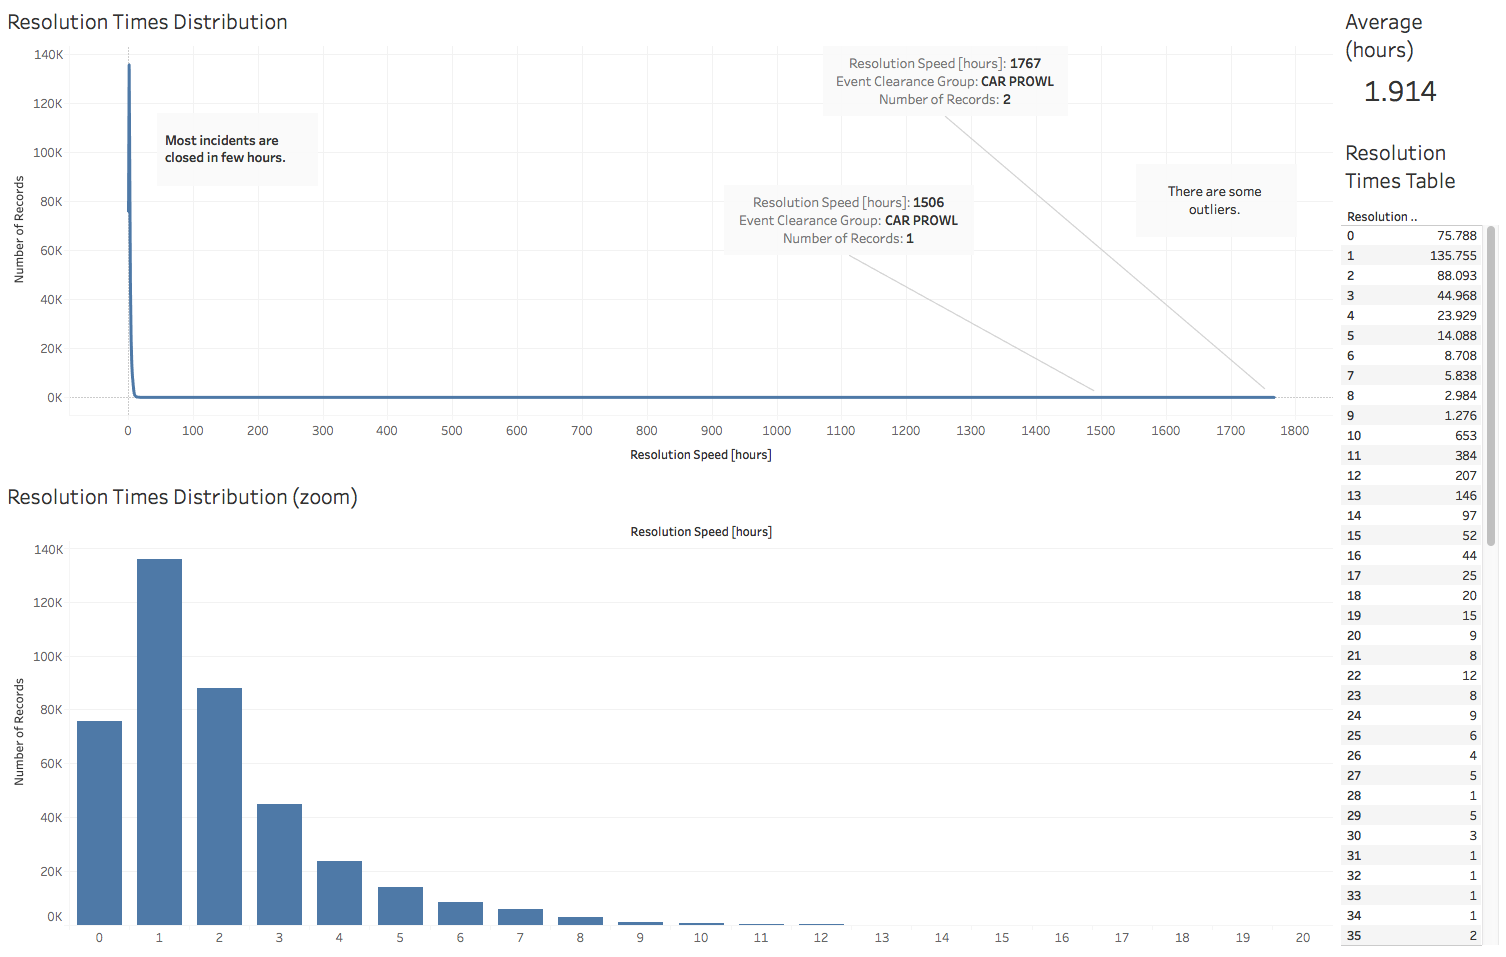
\includegraphics[width=\columnwidth]{figures/3_1_resolution_speed}
	\caption{Distribution of the resolution times. The dashboard is called ``Resolution Times'' in Tableau.}
	\label{fig:3_1_resolution_speed}
\end{figure}


\subsection*{Question 3.2}
\textit{Are there certain types of incidents having a much lower resolution speed than others? If so, which are these?}



\subsection*{Question 3.3}
\textit{Does the resolution speed depend on the time period (e.g., year, season of the year)?}
